\documentclass{report}

\usepackage{my_lab}

\begin{document}

\graphicspath{{figures}}

\LabTitle{3.2.8}{Релаксационные колебания}

% \tableofcontents
% \listoffigures
% \listoftables

\textbf{Цель работы}:
\begin{enumerate}
	\item изучение вольт-амперной характеристики нормального тлеющего разряда
	\item исследование релаксационного генератора на стабилитроне
\end{enumerate}

\textbf{Приборы}:
\begin{enumerate}
	\item стабилитрон СГ-2 (газонаполненный диод) на монтажной панели
	\item магазин ёмкостей
	\item магазин сопротивлений
	\item источник питания
	\item амперметр
	\item вольтметр
	\item осциллограф
\end{enumerate}

\section{Теоретические сведения}

\begin{figure}[H]
	\centering
	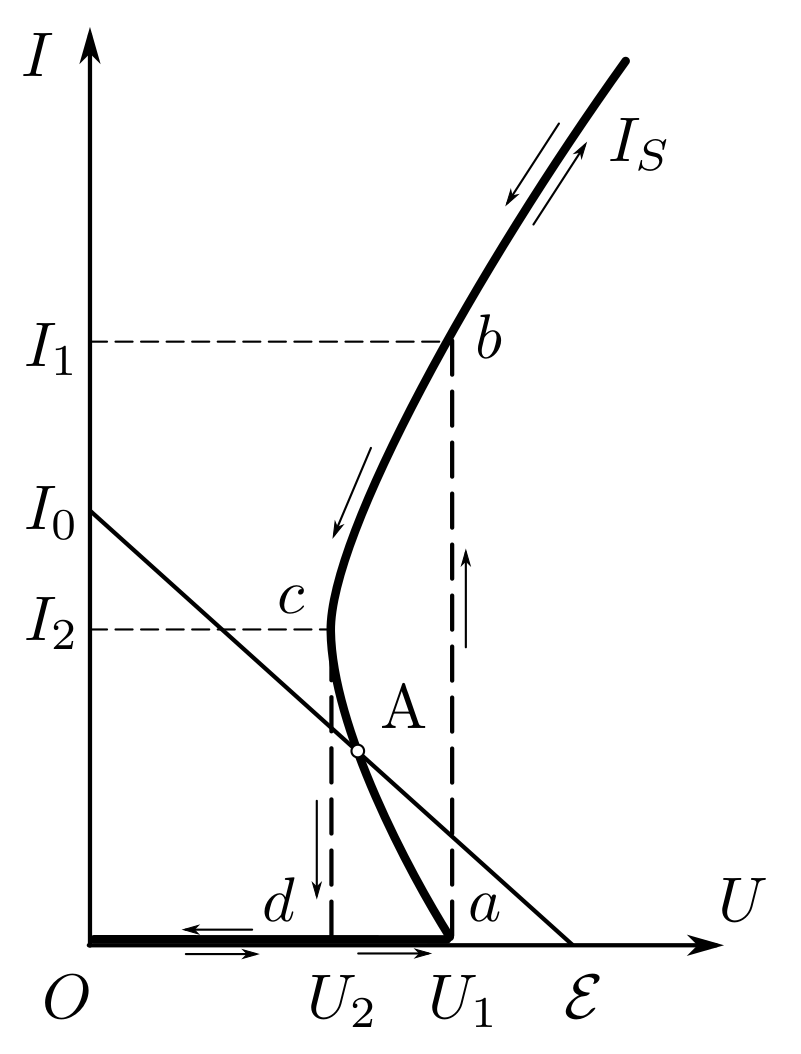
\includegraphics[width=0.4\linewidth]{VAH2}
	\caption{ВАХ газонаполненного диода}
	\label{fig:VAH}
\end{figure}

\begin{figure}[H]
	\centering
	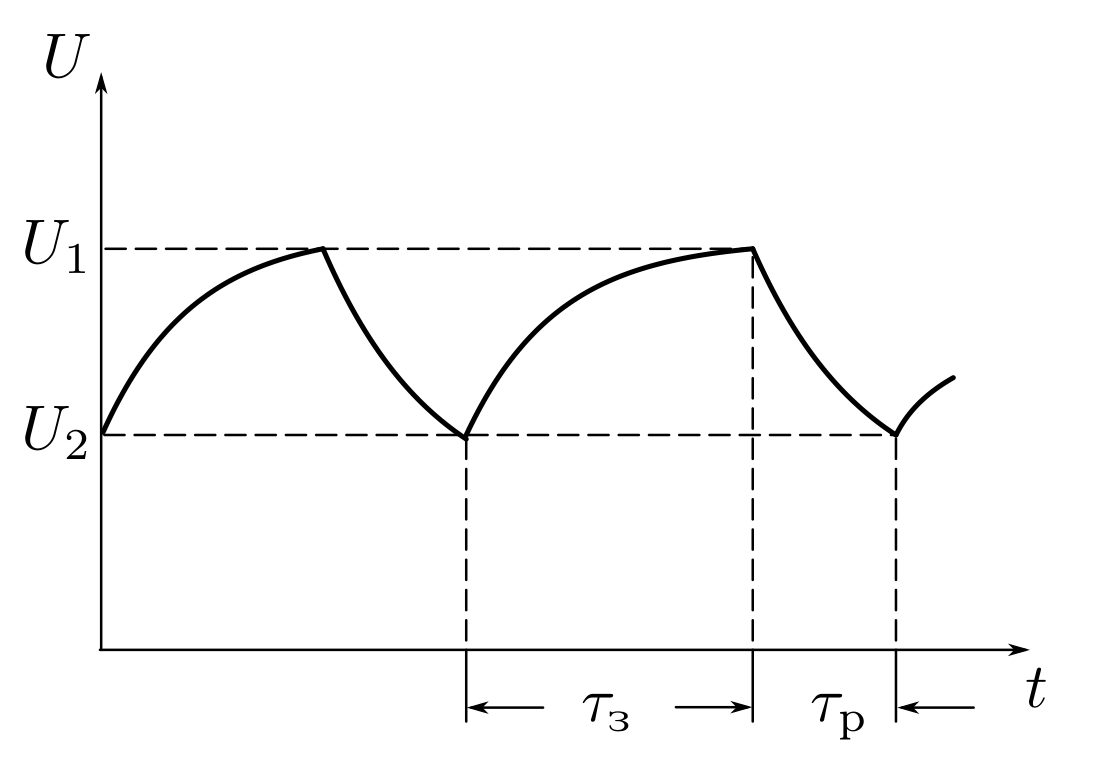
\includegraphics[width=0.4\linewidth]{U1}
	\caption{Осциллограмма релаксационных колебаний}
	\label{fig:VAH}
\end{figure}

\begin{figure}[H]
	\centering
	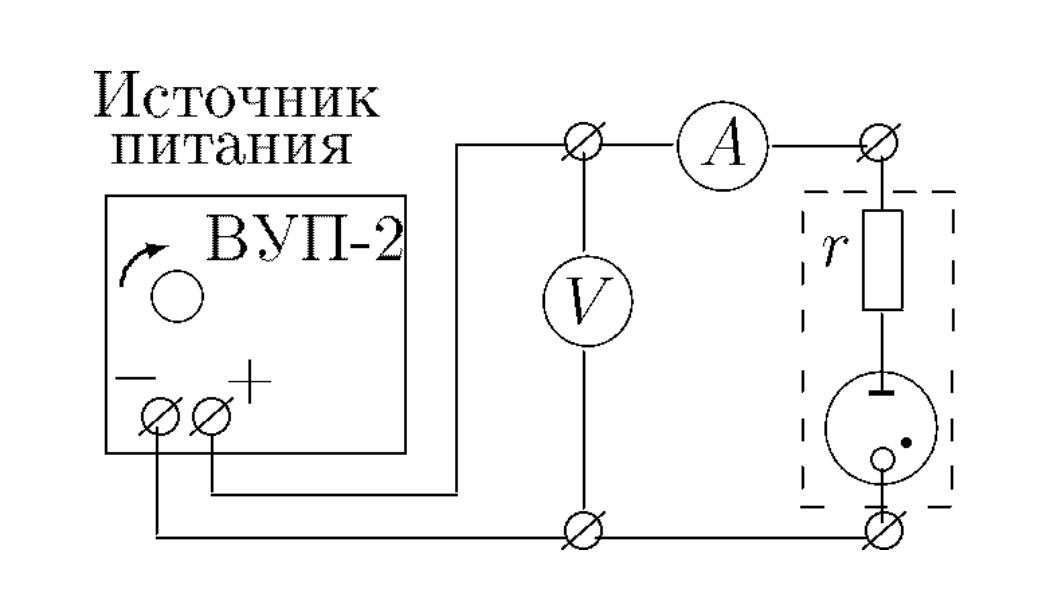
\includegraphics[width=0.6\linewidth]{Scheme1}
	\caption{Схема для исследования ВАХ}
	\label{fig:s1}
\end{figure}

\begin{figure}[H]
	\centering
	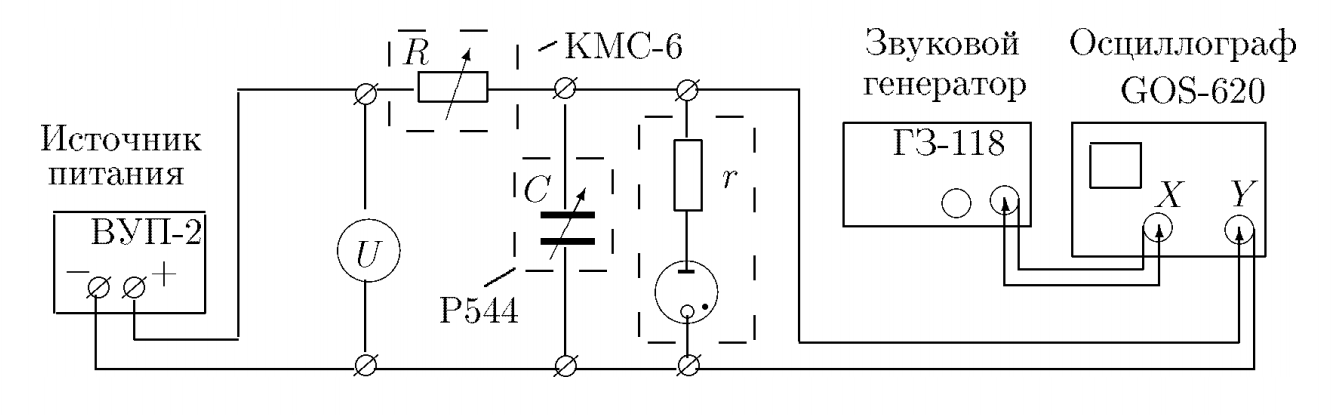
\includegraphics[width=0.8\linewidth]{Scheme2}
	\caption{Схема для исследования релаксационного генератора}
	\label{fig:s2}
\end{figure}

При стационарном режиме ($I, U = \mathrm{const} $),
\begin{equation}\label{k}
	I_{\text{ст}} = \frac{\varepsilon - U}{R + r}
\end{equation}

\begin{equation}\label{key}
	R C \frac{d U}{d t} = \varepsilon - U
\end{equation}
\begin{equation}\label{key}
	U = \varepsilon - (\varepsilon - U_2)\ \exp{\frac{-t}{R C}}
\end{equation}
В момент зажигания: $t = \tau_3,\quad U = U_1$:
\begin{equation}
	U_1 = \varepsilon - (\varepsilon - U_2)\ \exp{\frac{-\tau_3}{R C}}
\end{equation}
\begin{equation}
	T \approx \tau_3 = R C \ln{\frac{\varepsilon - U_2}{\varepsilon - U_1}}
	\label{eq:T}
\end{equation}

\section{Ход работы.}
\begin{enumerate}
	\item Соберем схему 1. (см. рис. \ref{fig:s1})
	      \[
		      r = 5.1 \kilo \Ohm
		      .\]
	\item Установим мин. напряжение.
	\item Получим ВАХ. (см. таблицу \ref{table:1})
	      \begin{table}[H]
		      \centering
		      \begin{tabular}{|l|l|}
			      \hline
			      U, $ \Volt $ & I, $ A $ \\
			      \hline
			      25           & 0        \\
			      43           & 0        \\
			      65           & 0        \\
			      69           & 0        \\
			      72           & 0        \\
			      93           & 0        \\
			      93           & 4        \\
			      97           & 5        \\
			      99           & 4        \\
			      102          & 6        \\
			      105          & 6        \\
			      116          & 8        \\
			      127          & 10       \\
			      139          & 13       \\
			      159          & 16       \\
			      184          & 21       \\
			      206          & 25       \\
			      234          & 30       \\
			      262          & 36       \\
			      331          & 45       \\
			      \hline
		      \end{tabular}
		      \hspace{1cm}
		      \begin{tabular}{|l|l|}
			      \hline
			      U, $ \Volt $ & I, $ A $ \\
			      \hline
			      313.0        & 45.5     \\
			      263.0        & 36.9     \\
			      225.0        & 28.9     \\
			      196.0        & 23.4     \\
			      171.0        & 18.7     \\
			      145.3        & 13.9     \\
			      125.0        & 10.1     \\
			      109.3        & 7.1      \\
			      94.7         & 4.4      \\
			      84.7         & 2.4      \\
			      82.6         & 2.0      \\
			      80.6         & 1.6      \\
			      79.7         & 1.5      \\
			      78.5         & 1.2      \\
			      76.9         & 0.9      \\
			      75.0         & 0.6      \\
			      74.0         & 0.4      \\
			      73.6         & 0.0      \\
			      72.9         & 0.0      \\
			      71.3         & 0.0      \\
			      67.2         & 0.0      \\
			      30.0         & 0.0      \\
			      \hline
		      \end{tabular}
		      \caption{ВАХ стабилитрона}
		      \label{table:1}
	      \end{table}
	      \begin{gather}
		      U_1 \approx 93 \Volt\\
		      U_2 \approx 74 \Volt
	      \end{gather}
	\item Соберем схему 2. (см. рис. \ref{fig:s2})
	\item Установим на магазине ёмкостей значение $C = 50 \nano \Farad$, а на
	      магазине сопротивлений $R = 900 \kilo \Ohm$.
	\item Подсоединим осцилограф и установим $ \varepsilon \approx 1.2 U_1 $.
	      \[
		      \varepsilon = 112\ \Volt
		      .\]
	\item Подберем частоту осциллографа так, чтобы были видны колебания на
	      конденсаторе (канал 1) и на стабилитроне (канал 2).
	\item По графику "пилы" оценим $ \tau_3, \tau_p, T, \nu $.
	      \begin{gather}
		      \tau_3 = 35.5 \mili \sec \\
		      \tau_p = 1.5 \mili \sec \\
		      T = 37 \mili \sec \\
		      \nu = 27 \Hz
	      \end{gather}
	\item Найдем $ R_\text{кр} $, уменьшая $ R $.
	      \begin{equation}
		      R_\text{кр} = 150 \kilo \Ohm
	      \end{equation}
	\item Убедимся, что колебаня пропадают и при уменьшении $ \varepsilon $.
	\item Измерим зависимость $ T(C),\quad C \in [2, 50] \nano \Farad $.
	      (см. таблицу \ref{table:2}).
	      \[
		      R_0 = 450 \kilo \Ohm
		      .\]
	      \begin{table}[H]
		      \centering
		      \begin{tabular}{|l|l|}
			      \hline
			      C, $ \nano \Farad $ & T, $ \mili \sec $ \\
			      \hline
			      50                  & 31                \\
			      45                  & 27                \\
			      40                  & 25                \\
			      35                  & 21                \\
			      30                  & 19                \\
			      25                  & 15                \\
			      20                  & 13                \\
			      15                  & 9                 \\
			      10                  & 7                 \\
			      5                   & 3                 \\
			      \hline
		      \end{tabular}
		      \caption{T(C)}
		      \label{table:2}
	      \end{table}
	\item Измерим зависимость $ T(R),\quad R \in [R_{\text{кр}}, R_{max}]$.
	      (см. таблицу \ref{table:3}).
	      \[
		      C_0 = 50 \nano\Farad
		      .\]
	      \begin{table}[H]
		      \centering
		      \begin{tabular}{|l|l|}
			      \hline
			      R, $ 10^5 \Ohm $ & T, $ \mili\sec $ \\
			      \hline
			      10               & 68               \\
			      8                & 54               \\
			      7                & 46               \\
			      6                & 40               \\
			      5                & 33               \\
			      4                & 26               \\
			      3                & 20               \\
			      2                & 14               \\
			      \hline
		      \end{tabular}
		      \caption{T(R)}
		      \label{table:3}
	      \end{table}
	\item Восстановим работу релаксационного генератора (рис. \ref{fig:s2}) с настройками, рекомендованными в п. 5–6.
	\item Переведем осциллограф в
	      измерительный двухканальный режим. Установм по осям координат
	      сдвиги и коэффициенты усиления, подходящие для наблюдения фазовой
	      траектории релаксационных колебаний.

	      Должны получится фигуры Лиссажу.
	\item
	      Не выполняли.
	\item Построим графики ВАХ.
        \begin{figure}[H]
            \centering
            \includesvg[width=1\linewidth]{figures/I1(U).svg}
            \includesvg[width=1\linewidth]{figures/I2(U).svg}
        \end{figure}
	\item Построим графики $ T_\text{эксп}(C), T_\text{теор}(C) $ и $ T_\text{эксп}(R), T_\text{теор}(R) $.\\
	      По ур-ию \ref{eq:T}:
	      \begin{equation}
		      T \approx R C \ln{\frac{\varepsilon - U_2}{\varepsilon - U_1}}
	      \end{equation}
	      \[
		      \varepsilon = 112,\quad U_1 \approx 93,\quad U_2 \approx 74,
		      \quad R_0 = 450 \kilo\Ohm,\quad C_0 = 50 \nano\Farad
	      \]
	      \[
		      \ln{\frac{\varepsilon - U_2}{\varepsilon - U_1}} \approx 0.7
	      \]
	      \begin{gather}
		      T_\text{теор}(C) \approx 0.2 \frac{\mili\sec}{\nano\Farad} \cdot C \\
		      T_\text{теор}(R) \approx 3.5 \frac{\mili\sec}{10^5 \Ohm} R
	      \end{gather}

	      \begin{figure}[H]
		      \centering
		      \includesvg[width=1\linewidth]{figures/T(C).svg}
	      \end{figure}
	      \begin{figure}[H]
		      \centering
		      \includesvg[width=1\linewidth]{figures/T(R).svg}
	      \end{figure}

	      \begin{gather}
		      T_\text{эксп}(C) \approx 0.6 \frac{\mili\sec}{\nano\Farad} \cdot C \\
		      T_\text{эксп}(R) \approx 6.8 \frac{\mili\sec}{10^5 \Ohm} R
	      \end{gather}
	\item
	      Эксперементальные значения стабильно выше, чем теоритические.
	      Как было сказано выше, данная систематическая погрешность может быть
	      связана с пренебрежением паразитных емкостей и индуктивностей схемы,
	      отличие $ U_2 $ от реального потенциала гашения лампы.

	      Оченим потенциал гашения.
	      \begin{gather}
		      V \approx 40 \Volt
	      \end{gather}

	\item
	      Не выполняли.
	\item
	      Не выполняли.
\end{enumerate}

\section{Вывод.}
В данной лабораторной работе мы получили ВАХ нормального тлеющего затяда и
исследовали релаксационный генератор на стабилитроне.
Получили напряжение зажигания $ U_1 $ и напряжение гашения $ U_2 $:
\begin{gather}
	U_1 \approx 93 \Volt\\
	U_2 \approx 74 \Volt
\end{gather}
Получили зависимости $ T(C) $ и $ T(R) $, построили графики.
Из результатов видно, что динамический потенциал гашения
значительно меньше статического напряжения гашения. В пределах применения
теоретической модели наблюдается прямопропорциональная зависимость периода от
сопротивления и емкости.

\end{document}
